\section{آشنایی با مشخصه i-v یک دیود}

\subsection{الف)}
\begin{figure}[h]
    \centering
    \fbox{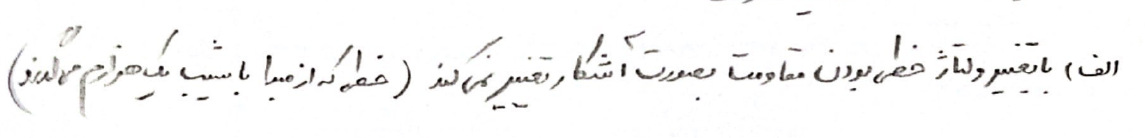
\includegraphics[width = \textwidth]{Q6/pishAlef.png}}
    \caption{\textcolor{blue}{از پیش گزارش داریم}}
\end{figure}
طبق داده هایی که در آزمایشگاه گرفتیم.\\
\begin{latin}
    \begin{table}[h]
        \centering
        \begin{tabular}{|c|c|c|c|c|c|c|}
            \hline
            V(V)  & 0.8  & 1.6  & 2.5  & 3.2 & 4    & 5   \\
            \hline
            I(mA) & 0.89 & 1.63 & 2.56 & 3.2 & 4.05 & 5.1 \\
            \hline
        \end{tabular}
        \caption{measured values}
    \end{table}
\end{latin}
\begin{figure}[h]
    \centering
    \fbox{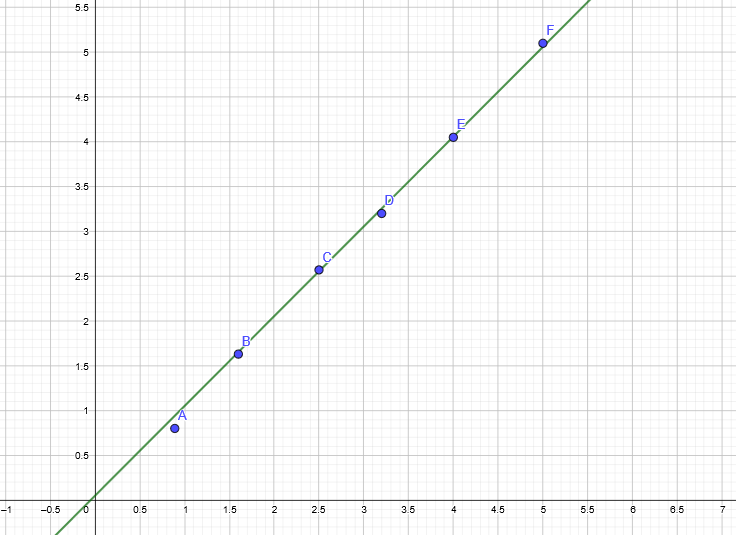
\includegraphics[width = 0.8\textwidth]{Q6/alefNemudar.png}}
    \caption{نمودار}
\end{figure}
با تحلیل بدست میاریم که $$B=1.002,A=0.05,r=0.9998$$
\pagebreak
\subsection{ب)}
\begin{figure}[h]
    \centering
    \fbox{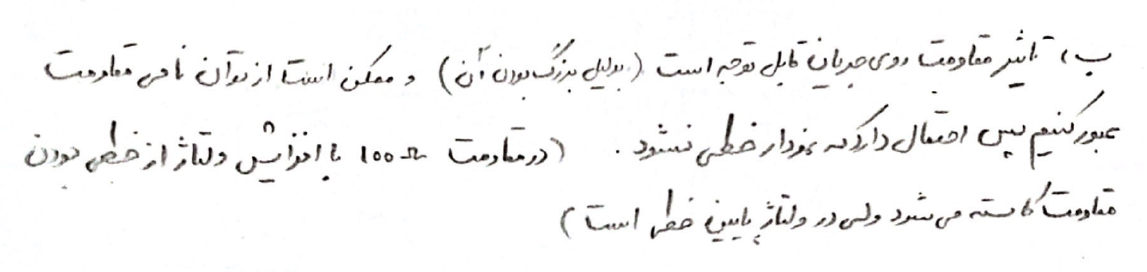
\includegraphics[width = \textwidth]{Q6/pishB.png}}
    \caption{\textcolor{blue}{از پیش گزارش داریم}}
\end{figure}
\pagebreak
\subsection{ج)}
\begin{figure}[!h]
    \centering
    \fbox{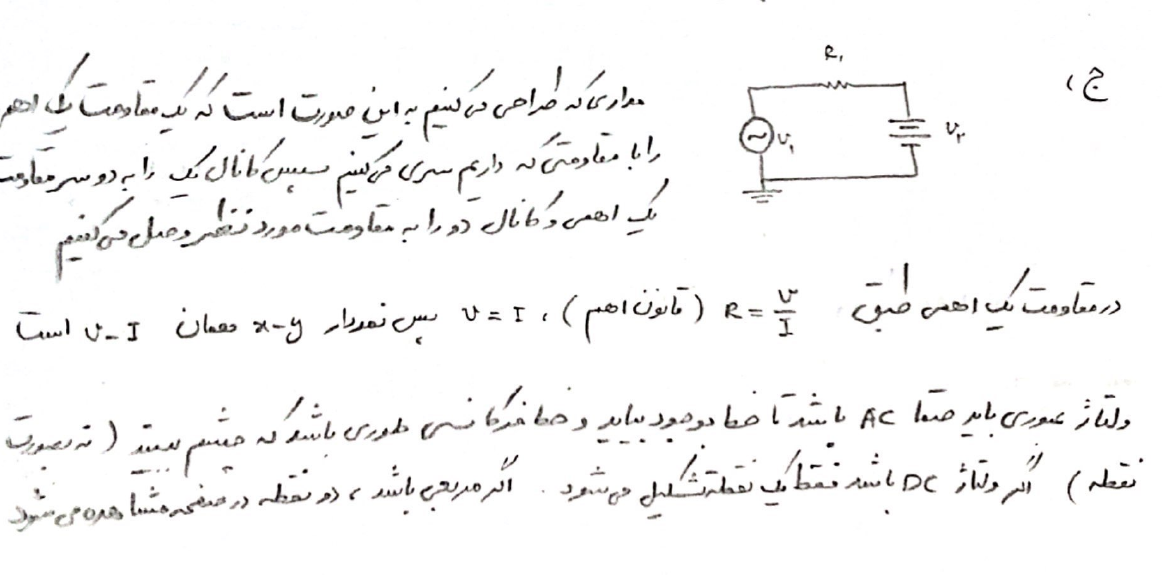
\includegraphics[width = 0.8\textwidth]{Q6/pishJ.png}}
    \caption{\textcolor{blue}{از پیش گزارش داریم}}
\end{figure}
\begin{figure}[h]
    \centering
    \fbox{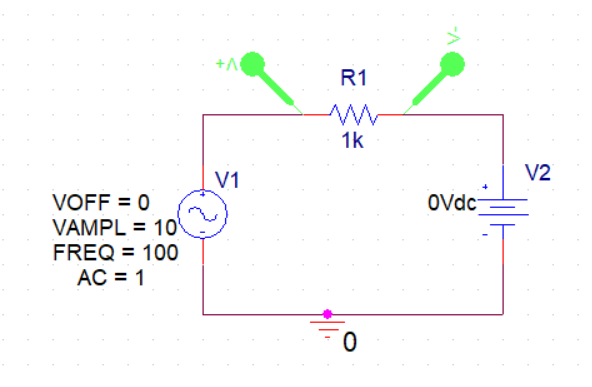
\includegraphics[width = 0.45\textwidth]{Q6/pSpiceMadar.png}}
    \fbox{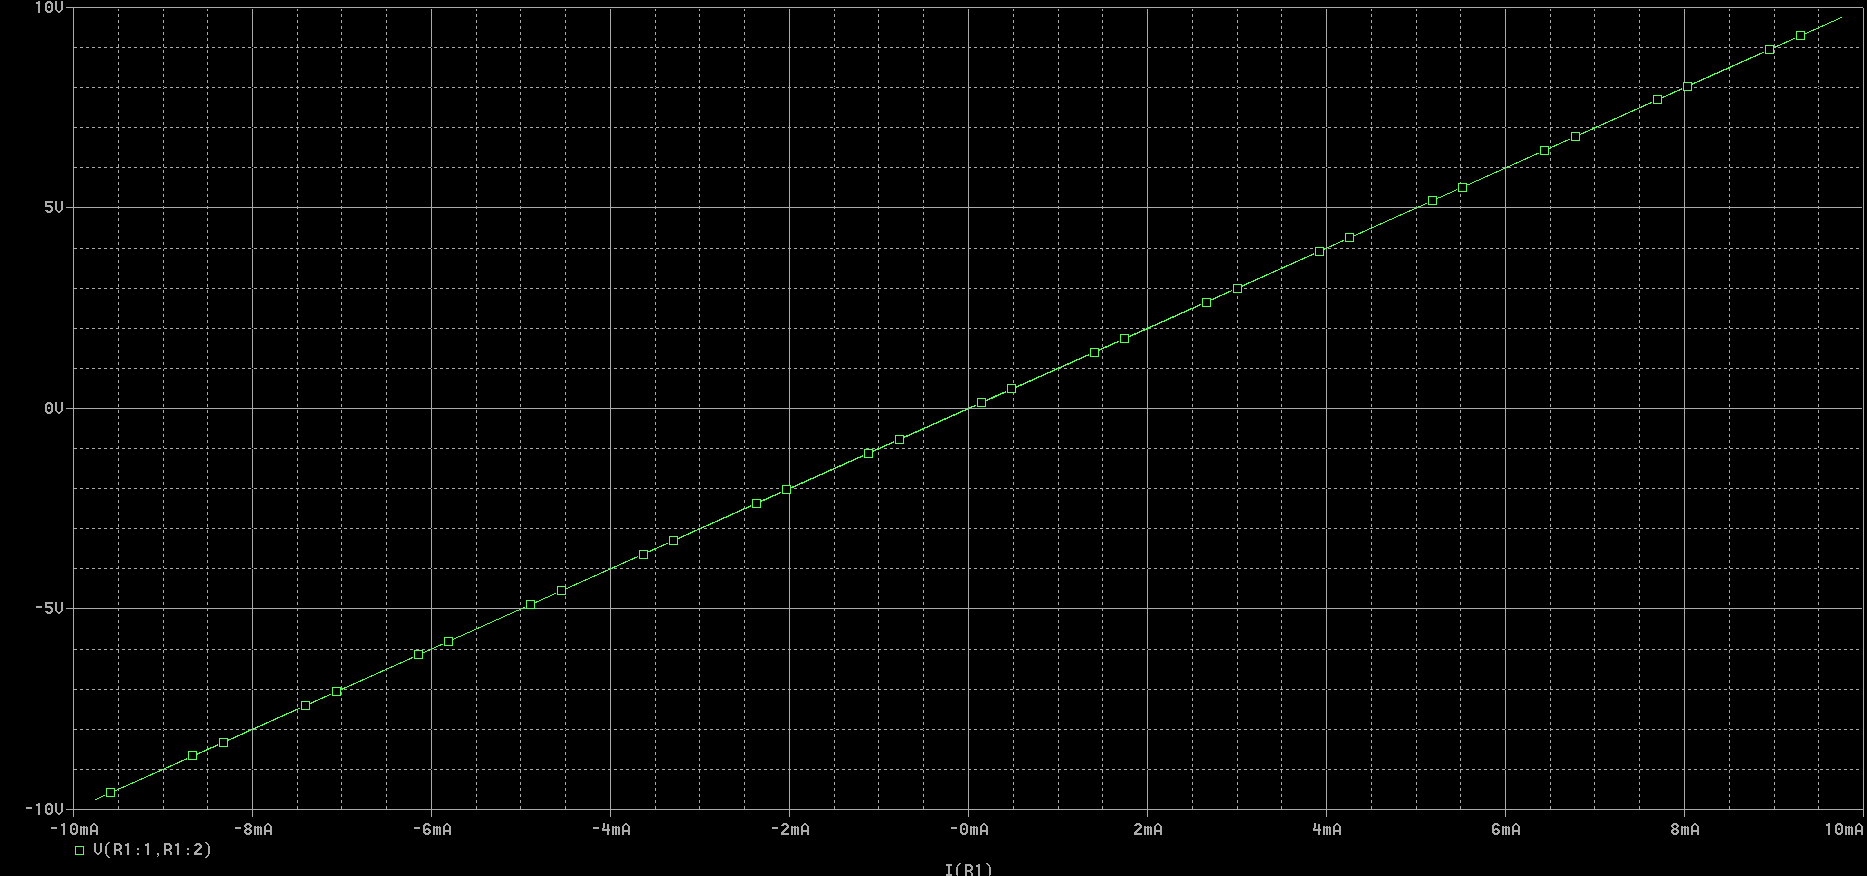
\includegraphics[width = 0.45\textwidth]{Q6/pSpiceNemud.png}}
    \caption{شبیه سازی با اسپایس}
\end{figure}
همه چیز مورد انتظارمان بدست میاید.
\pagebreak
